%
% 












\subparagraph{Work Package 2 - Access to RIs for Physics}

The scientific projects conducted by the WP2 TA users were concentrating on two frontiers: studying extremes in nature and the precision frontier. In many experimental approaches the complementarity of the WP2 facilities plays the crucial role.

\textbf{The advancing of core principles by studying extremes in nature}\\ 
In WP2, this challenge is faced by creating and probing nuclei under controlled conditions and studying nuclei that exist only in unimaginably vast bodies (10$^{25}$m) like stars and galaxies, thus connecting their properties to the physics of very small systems (10$^{-15}$m). 
%WP3 and WP4 give the necessary tools to go down to even smaller length %scale.  
Elucidating the behavior of nuclei at the femtometer scale requires a study over a wide range of nuclei, %akin to needing to 
similar to the need of a full DNA sequence rather than a DNA fragment to understand a disease. The experiments with various instrumentation at the WP2 facilities, along with charged stable beams (2.1), short-lived radioactive beams (2.2) and neutron beams (2.3)  do exactly this. In the P2 reporting period, insights into questions ranging from the existence (and production) of nuclei at the extremes in charge and mass number (and very asymmetric nuclear matter), understanding where and how did the elements from iron to uranium originate,
%what are the limits of the periodic table 
to physics beyond the standard model, were gained. State of art spectrometers of different specification storage rings, detectors ranging from high-resolution Advanced Gamma tracking array to charged particle arrays (among large Pan European collaborations), coupled with beams over a broad energy range, from 1 MeV/u to 1 GeV/u, have been exploited to explore the phase space of Excitation Energy, Angular momentum and Isospin. 

\textbf{The precision frontier}\\
Precise measurements of nuclear life times of excited states, to probe octupole shapes in rare earth nuclei, shape coexistence, breakdown of conventional “magic” numbers far from the valley of stability in various parts of the Segré chart, have been made (concerning the first shell closure arising from the spin orbit coupling (N= 28), N=50, 82 and N=126, the latter being a critical region for the r-process in nucleosynthesis). Precision measurements of the masses relevant to astrophysical model calculations were also performed. Today in nuclear physics the precision of mass measurements  is 1 in 10$^{13}$. Storage rings have also been used to study electron screening effects which currently 
affect astrophysical rate calculations. Using radioactive ion beams and an active target, reactions relevant to nucleosynthesis, from the early stage to the r-process, have been measured. New sensitive Laser spectroscopy tools, coupled with atomic and solid state coupling constant (hyperfine structure) have also been used to study nuclear structure effects on Gamma ray strength functions, ranging from low lying “pygmy" dipole resonances to understanding neutron “skins” and highly hindered transitions. 
Isospin symmetry breaking and role of neutron-proton pairing is also being explored through nuclear excitations. The path to produce very heavy and very neutron rich systems through fusion-evaporation is extremely challenging, so work to probe new mechanisms of Multi-nucleon transfer has been explored.  In precise experiments involving nuclear beta decay using polarised nuclei,  the time-violating D triple correlation coefficient were measured, relating the
spin of the nucleus and neutrino and electron momenta. These measurements give  independent limits compared to those obtained from colliders on physics beyond the standard model.

\textbf{Complementarity of the facilities}\\
Complete isotopic distributions of fission products, not yet known,  were measured both with high and low energy stable and radioactive ion beams. Thanks to improvements in spectrometers, these results are important for next generation fission reactors. On the other hand, the effect of gas production in Chromium and Copper in Materials for fusion reactors  was studied using neutron beams. Neutron beams were also used for measuring the activity of actinides in Baltic seawater, with techniques for refined fast neutron tomography. The effect of high neutron fluence on scintillating detectors, to be employed in experiments designed toaccess the nuclear matrix elements entering the expression of the double beta decay lifetime, were tested. More details are given in the following three sections related to the use of stable, radioactive and neutron beams to investigate the many facets of the nuclear many-body quantum problem, relevant to basic and applied science.

The studies in WP2 mainly investigated properties of nuclei not existing on earth (exotic nuclei), to improve our understanding of their internal structure and reaction mechanisms, and our knowledge of the nuclear interaction. 
This research has an impact on the modeling of astrophysical scenarios, as well as on applications, detector characterization and interdisciplinary research. 

\subparagraph{Task 2.1: Stable Ion Beams} \mbox{}

At \textbf{GANIL}, there were two main themes in the studies carried out by the nuclear physics community – fission and nuclear structure in exotic systems. 

Complete isotopic fission yields from inverse kinematics transfer-induced fission in the thorium region were studied. Isotopic identification of fission fragments emitted from a number of fissioning systems produced by transfer reactions between a $^{232}$Th stable beam (new GANIL beam) and a 
Carbon target was performed through the measurement of the target-like recoil in the Particle Identification Silicon Telescope Array (PISTA) detector.  The origin and competition between fission modes in the pre-actinides was studied, in the transitional case of $^{192}$Po. The recent observation of a new asymmetric-fission “island”, located in the neutron-deficient pre-actinide region south-west of $^{208}$Pb, revealed the important role of additional, unforeseen, microscopically driven favored proton configurations. 

%While the transition from symmetric to asymmetric fission with increasing mass in actinides has been studied in detail, the transition from symmetric to asymmetric fission with decreasing mass in pre-actinides has not yet been mapped. The experiment aimed to collect such new data for neutron deficient pre-actinides, to track the transition from asymmetric to symmetric fission in the region and connect it to the actinide island.

Nuclear structure in exotic systems was studied in several experiments. Spin-orbit splitting in the N = 19 isotones was studied in 
the direct transfer reaction p($^{34}$Si,$^{33}$Si)d, with a secondary radioactive $^{34}$Si beam at an energy of 50 MeV/u, provided by LISE from the fragmentation of a $^{36}$S stable primary beam, impinging on a CH2 target. The detection set-up was composed of MUGAST + EXOGAM + Zero-Degree Detection. The cluster structure of the ground-state of light neutron-rich nuclei, beyond alpha-clustering, was investigated. The $^{10}$Be(d,$^6$Li)$^6$He cross-section was measured in order to check the consistency between the transfer and knockout reaction approaches, as the $^{10}$Be(p,p$\alpha$) cross-section was previously measured at RIKEN.   The g-factor of the first 2$^+$ excited state in $^{22}$Ne was measured, of significant importance for two reasons: (i) the g-factor of this stable nucleus is of great theoretical interest, and (ii) although a high-precision value (~2$\%$) had been previously reported, it was called into question following measurements at ISOLDE on $^{28}$Mg. A highly accurate determination of g(2$^+$) in $^{22}$Ne will clarify the discrepancy and aid in the interpretation of data obtained for radioactive $^{28}$Mg from ISOLDE. Preliminary results already indicate that the previously reported high-precision value deviates by several sigma from the current observations.

At \textbf{GSI}, currently a topic of investigation across the community, Multi Nucleon Transfer (MNT) reactions at the Coulomb barrier offer a promising route to produce unknown neutron-rich nuclei and possibly access the super heavy mass region. A new method combining a high-resolution TOF spectrometer (TOSCA) with a linear microcalorimeter (measuring kinetic energy) was tested. Precise $\Delta$E measurements behind a homogeneous solid absorber allow complete A and Z identification. Continuing the high profile and high impact measurements of the structure of heavy elements, laser spectroscopy studies of californium, fermium, nobelium, and lawrencium %continue efforts 
aim
to probe nuclear structure near N=152 and Z=100. The established RADRIS technique and the high-resolution JetRIS method were used to expand level searches and investigate ground and isomeric states, such as the K-isomer in $^{254}$No thereby refining modern nuclear models. As astronomical observations of primordial deuterium reach ultra-high precision, reducing uncertainties in Big Bang Nucleosynthesis (BBN) becomes crucial. A study of electron screening effects, which currently remain inadequately understood and affect reaction rate calculations in astrophysical scenarios have been studied at CRYRING. This was enabled by measuring the D(D,n)$^3$He and D(D,p)$^3$H reactions at energies below 0.4 MeV/A using the CARME array.

At the \textbf{IFIN-HH Tandem Accelerator Complex}, two experiments can be highlighted here. 
Octupole collectivity in $^{150}$Gd was studied at the ROSPHERE spectrometer in two complementary experiments aimed at measuring the lifetime of the 3$^-$ and 5$^-$ states using the recoil distance Doppler shift (RDDS) method and measuring the weak E3 transition branching ratios of these states populated in beta decay. A $^{13}$C beam incident on a thin $^{140}$Ce target was used to populated excited states in $^{150}$Gd in the RDDS experiment while a $^6$Li beam was used to produce radioactive $^{150}$Tb in order to study the beta decay to $^{150}$Gd. The combined experimental data showed increased B(E3) values, in particular the measured B(E3;3$^-$$\rightarrow$0$^+$)=45(5) W.u. being the highest and most precise octupole strength in the rare-earth region. This work 
was published in Phys. Rev. Lett. (\url{https://doi.org/10.1103/PhysRevLett.134.092501}) and Phys. Rev. C (\url{https://doi.org/10.1103/PhysRevC.111.034302}).
Gamma-ray strength functions and nuclear level density in $^{112,114}$Sn were studied for the first time using the Oslo method. Thermodynamic properties and the structure of the pygmy dipole resonance were extracted and compared with existing data in the Sn isotopic chain. The results are compared with microscopic models implemented in the TALYS reaction code and the fully microscopic quasiparticle-phonon model for the underlying nuclear structure of the dipole strength in $^{112,114}$Sn. This work was submitted for publication in Phys. Rev. C. 

At \textbf{JYFL}, one experiment used the TOSCA two-arm time-of-flight spectrometer to study fission dynamics at the Large Scattering Chamber (NRO155). All remaining experiments employed the recoil separators RITU and MARA, and concentrated on studies of isospin symmetry in N=Z nuclei and measurements of nuclear excited state lifetimes using the APPA plunger device. Lifetimes were measured successfully in $^{94}$Rh, $^{86}$Mo and $^{62}$Ga. A further highlight from these studies was the first attempt to measure lifetimes in the N=Z nucleus $^{66}$As, which is an extremely challenging case with current state-of-the-art instrumentation. A first attempt was also made at in-beam spectroscopy of $^{114}$Ba, another very challenging case, because of the production cross section and difficulty to cleanly extract the channel of interest. At RITU, which is designed for studies of heavier nuclei, highlights included the measurement of lifetimes in $^{179}$Au and $^{192}$Pb (addressing questions in nuclear shape co-existence) and two experiments exploring the potential to use Multi-Nucleon Transfer reactions to study nuclei inaccessible by other means.


At \textbf{INFN-LNL}, by the use of AGATA-SPIDER, a number of Coulomb excitation experiments were performed, for example to study the emergence of collectivity near $^{60}$Ni %(experiment 23.008) 
and the interpretation of the structure of excited 0$^+$ states in $^{106}$Pd. %(experiment 23.054).
AGATA-PRISMA was used, along with RDDS and DSAM techniques to measure lifetimes in $^{50-52}$Ca and $^{46-48}$Ar with the aim of  understanding shell evolution close to N=28 and Z=20. The same devices were used to measure Multi-Nucleon Transfer (MNT) reactions. In the first experiment, the MNT reaction mechanism was investigated in the $^{130}$Te + $^{208}$Pb system, 
%(experiment 23.064), 
whilst in the second, MNT was used as a tool to populate and study the structure of nuclei in the island of inversion from the reactions of $^{26}$Mg beam on a $^{238}$U target. Other devices combined with AGATA for experiments were AGATA-SAURON, AGATA-EUCLIDES and AGATA-OSCAR. These activities show the versatility of the devices which can be modified for campaigns of experiments using different complementary techniques.


At \textbf{NLC-CCB} two projects were conducted. The main objective of one measurement was to study the Pygmy Dipole Resonances (PDR) in stable nickel isotopes with proton beam and a high efficiency detector system, to disentangle the paradigm of neutron skin oscillations and future application to nuclear astrophysics. The $^{58}$Ni and $^{62}$Ni nuclei were excited using inelastic scattering of 180 MeV protons. The high energy gamma rays emitted from the decay of excited nuclei were detected, using 4 high efficiency LaBr$_3$ scintillators and 26 PARIS phoswiches, in coincidence with scattered protons measured by KRATTA array. 
The aim of the second  experiment was to study the decay of the M4 resonance state in $^{12}$C located at 19.5 MeV, by employing the 135-MeV proton inelastic scattering reaction, employing similar instrumentation as in the first experiment with added four Double-Sided Silicon Strip Detectors for light charged particles measurement, equipped with new, digital, read out.
%The objectives of the experiment were following: i) $^{12}$C(p,p') measurement at 135 MeV with thick, 150 mg/cm$^2$, $^{12}$C target for collecting the coincidence data between inelastically scattered protons, exciting the resonance, and gamma rays emitted from the decay products, ii) implementation and commissioning of the system of four Double-Sided Silicon Strip Detectors for light charged particles measurement, equipped with new, digital, read out, iii) $^{12}$C(p,p') measurement at 135 MeV with thin, 1 mg/cm$^2$, $^{12}$C target for recording the coincidences between inelastically scattered protons and light charged particles (protons, alphas) from the decay of the resonance. 

At \textbf{NLC-SLCJ} the EAGLE-NEDA-DIAMANT setup was employed in an experiment aimed at observing $\gamma$-ray radiation emitted from excited states of $^{57}$Cu. 
%which has only one valence proton outside the doubly magic, self-conjugate N=Z=28, $^{56}$Ni core. 
The N=Z=35 nucleus $^{70}$Br was studied to identify members of the T=1 isobaric analog states in $^{70}$Br with its even-even $^{70}$Se partner, in order to solve the puzzle of 
%The $^{70}$Br/$^{70}$Se isobar pair shows a unique behavior, with the Coulomb energy difference (CED) decreasing gradually with spin. Such an effect could be associated with significant shape changes with increasing angular momentum. However, 
the anomaly in the CED between the $^{70}$Br/$^{70}$Se isospin T=1 states.
%remains a puzzle due to the lack of experimental data for $^{70}$Br. The goal of the experiment was to establish the position of the 6$^+$ and 8$^+$ states, which would help to understand the CED in the $^{70}$Br/$^{70}$Se isobar pair, as such a negative trend is not observed elsewhere. 
Also gamma-ray spectroscopic experiments were carried out to study excited states in $^{134}$Sm and to search for wobbling bands in $^{103}$Pd and $^{101}$Ru.
Reaction dynamics was investigated in an experiment dedicated to studying the influence of dissipation, due to transfer channels, on fusion barrier distributions. The systems studied were $^{20}$Ne+$^{92,94,95}$Mo at several beam energies. 
%The masses of the products were identified using the Time-of-Flight (ToF) method. 
Preliminary results indicate that transfer mechanisms leading to the masses A=19 and 16 were the main transfer channels in all three systems, but in the case of $^{95}$Mo, a neutron pick-up transfer (A=21) also occurred. The experiment should clarify the influence of such transfer channels on the different structures of the barrier distributions.
The absolute transition strength between yrast levels in $^{172}$Os from level lifetimes measured with the recoil distance Doppler-shift (RDDS) technique and the Cologne plunger device, coupled to the EAGLE gamma-ray spectrometer was measured. 
%Gamma-gamma coincidences were employed to rule out any contribution from unobserved side-feeding of the levels of interest, thus allowing for the unambiguous determination of the respective level lifetimes. 
A preliminary analysis of the data indicates that the lifetimes of the lowest yrast state in $^{172}$Os up to at least the 8$^+$ state can be determined.

In task 2.1, a number of the achievements of user groups from period 2 were referred to above, with the majority of groups now carrying out analysis on the data sets obtained. It is certain that in coming years a large number of publications and other outputs will result. Here we choose to select one highlight, which emphasises the complementarity of the WP2 facilities. 
The question of the temperatue dependence of the E1 strength below the Giant Dipole Resonance (GDR), so called Pigmy Dipole Resonance (PDR), is of paramount interest for the understanding of nuclear structure, testing theoretical models and has important implications in astrophysics. A series of experiments addressing this question were conducted in the isotopic chain of Ni isotopes going from the N=Z $^{56}$Ni up to the exotic nucleus $^{66}$Ni, and from zero to finite temperature. The measurements were done in the two EURO-LABS facilities IFIN-HH (Bucharest)) and NLC-CCB (Krakow). In the first one, a fusion evaporation reaction mechanism was used to create exited nuclei that emitted high energy gamma rays during the de-excitation process.
%registered and detected with a high efficient and high resolution 4$\pi$ array of Compton supressed scintillator and light charged particle detectors.  
For the very first time the extra yield below the GDR was observed at finite temperature in different Ni isotopes. In the second experiment, a complementary measurement by the same experimental group was carried out using inelastic proton scattering on stable nickel isotopes with the aim to investigate, for the first time in Ni isotopes, the PDR excitation 
%below and also above the neutron threshold 
at zero temperature. 
%The experiment used a particle detector array as well as high efficiency scintillators detectors from the PARIS array to measure high-energy gamma rays and disentangle their polarity. 
Both experiments were described in the presentations at the Zakopane Conference on Nuclear Physics and published ({\url{https://www.actaphys.uj.edu.pl/S/18/2-A33/pdf} and \url{https://www.actaphys.uj.edu.pl/S/18/2-A34/pdf}. The preliminary results of the \textbf{temperature dependence of the Pygmy Dipole Resonance} are shown in Fig.~\ref{fig:Wieland} }.

\begin{figure}[!h]
    \centering
    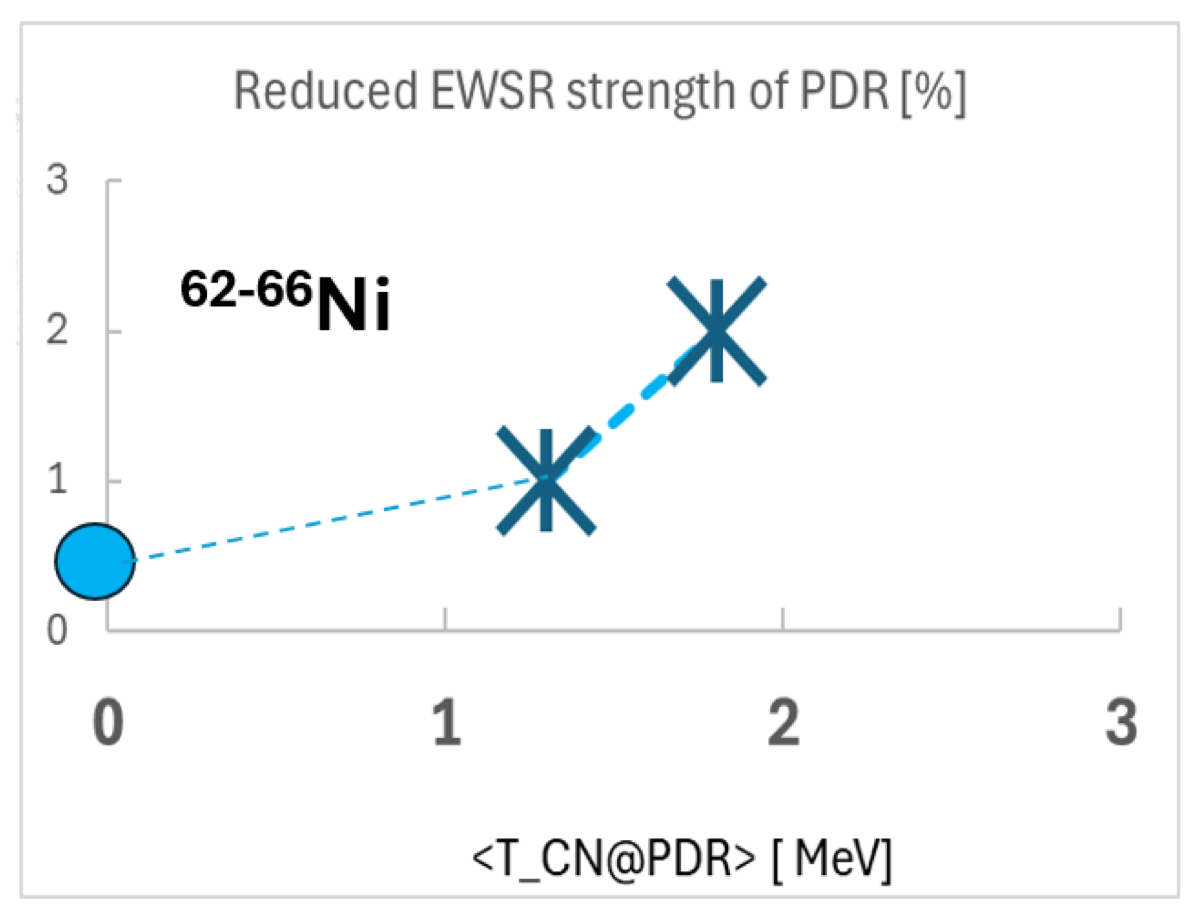
\includegraphics[width=0.6\linewidth]{graphics/Wieland.png}
    \caption{Combined preliminary results of the experiments done at CCB (circle) and IFIN (crosses). The plot shows the extra yield below the GDR for different Ni isotopes as a function of the nuclear temperature.
}
    \label{fig:Wieland}
\end{figure}


\subparagraph{Task 2.2: Radioactive Ion Beams} \mbox{}

At \textbf{GANIL-SPIRAL2} one project focused on $^{12}$Be structure in the vicinity of different cluster thresholds, such as $^4$He, $^7$He, $^8$He by searching for narrow resonances using ACTAR-TPC detector. Second project focused at indirectly quantifying $^8$Li($\alpha$,n)$^{11}$B reaction. This reaction is involved in the nucleosynthesis from the early evolutionary stage of our universe, till the starting of r-process nucleosynthesis in supernovae, collapsars and neutron star mergers. The study has been performed by understanding the compound nucleus for the reaction, the neutron-rich $^{12}$B, with the help of the resonant elastic scattering reaction $^4$He($^8$Li,$\alpha$)$^8$Li.

At \textbf{GSI/FAIR} experiments using FRS recorded a comprehensive dataset for projectile-fragmentation products (Z = 82 to 89) from $^{238}$U on a Be target, providing essential data to refine fragmentation models and support future NUSTAR experiments. ESR has been used for investigating the rare double-gamma decay mode in 0$^+$$\rightarrow$0$^+$ transitions; this study measured isolated double-photon decays in $^{72}$Ge, and compared the two-photon decay in $^{98}$Zr and $^{98}$Mo to assess whether enhanced transition rates depend on nuclear structure, and measures of de-excitation probabilities over a wide energy range in excited $^{238}$U and $^{239}$U. For the first time, simultaneous measurements of fission, gamma, and multi-neutron emission (up to three neutrons) were achieved in a storage ring setting. R3B setup has been used for commissioning of key detectors (CALIFA, Si-tracker FOOT, NeuLAND). Cross-section measurements for (p,pd) reactions on various carbon isotopes were performed indicating the presence of strongly correlated neutron-proton pairs, with quasi-deuteron behavior influencing nucleon “dressing” in the nuclear medium. DESPEC gathered spectroscopic data around N=126 shell closer, a critical region for r-process nucleosynthesis, where new level schemes and transition probabilities help benchmark models describing the interplay of single-particle orbitals and collective excitations in heavy nuclei relevant for the astrophysical sites. FRS Ion Catcher has been used in three different experiments. A proof-of-principle study using slowed-down uranium beams in a Cryogenic Stopping Cell demonstrated that multi-nucleon transfer (MNT) reactions can produce neutron-rich isotopes (A $\approx$ 160–250). MNT products were successfully extracted and identified with the MR-TOF mass spectrometer, paving the way for future RIB production at Super-FRS (cf. \url{https://doi.org/10.1016/j.nuclphysa.2025.123041}). Also focusing on exotic nuclei from Br to Rh, this study addresses issues such as isospin symmetry breaking, the Wigner effect, and unexpected mass discrepancies (e.g., $^{70}$Br). The FRS Ion Catcher, combined with a $^{107}$Ag fragmentation beam and SIS-18 accelerator mode, delivered precise mass measurements, essential for validating nuclear models and rp-process calculations. EXPERT detector, using a $^9$C beam, probes Thomas-Ehrman shifts in mirror pairs (e.g., $^5$H-$^5$Be, $^6$H-$^5$B, $^7$H-$^7$C) and measures decay energies, widths, and half-lives (down to picoseconds) via multi-particle angular correlations. Upgraded high-rate tracking detectors have enabled high-statistics data collection, allowing for improved measurements of nuclear state widths and the identification of novel multi-proton decay mechanisms.

At \textbf{JYFL}, by using a new beta detector at IGISOL made at NCNR (Swierk/Poland), trap-assisted decay spectroscopy of very neutron-rich Rh and Pd isotopes has been performed. An interesting experiment used a reaction of deuterons on $^{242}$Pu target(s), with the goal of producing both ground states and fission isomers in $^{240,242}$Am. Set of silicon detectors were installed in the switchyard, to be used for measuring alpha activity as well as fission fragments from the decay of the isomeric states. Operated in a “duty cycle mode”, with activity monitored in the switchyard as well as beam injected into the RF cooler, either for the MR-TOF or for JYFLTRAP. The latter allowed for separation of $^{242}$Am from the target $^{242}$Pu material. Half-lives were measured, total kinetic energy of the FFs as well as the excitation energy of $^{242f}$Am with the MR-TOF. Trap-assisted decay spectroscopy of fission fragments has been performed using a beta detector connected to a tape station and surrounded by a coaxial Ge and two large BeGe detectors. This setup allowed the collection of gamma-ray transitions with energy below 20 keV in A=115 isobars region. Another project focused on neutron-deficient Ag isotopes using collinear laser spectroscopy to provide a comprehensive data set that can be used to establish a precise and accurate reference quadrupole moment for the whole Ag chain. Combined with state-of-the-art atomic calculations the aim is to investigate the consistency of quadrupole moments deduced using atomic and solid-state crystal coupling constants. A second motivation was to determine the hyperfine anomaly in Ag, which reflects changes in the distribution of nuclear magnetization. 

At \textbf{CERN/ISOLDE} several experiments addressed very topical physics in nuclei around the $^{132}$Sn double shell closure. The $^{132}$Sn(d,p) reaction has underpinned the scientific cases of many different radioactive ion beam facilities, but only a single measurement existed from more than 15 years ago before a recent ISOLDE study. This experiment studied the reaction with around ten times the intensity of $^{132}$Sn, with a higher beam energy, and with a novel spectrometer giving much improved resolution. This revealed population of $all$ the valence single-neutron orbitals for the first time and their single-particle content has been deduced, establishing them all as carrying “full” single-particle strength. In parallel, $\beta$-delayed neutron decay studies at ISOLDE have also populated the 13/2$^+$ state, with even higher energy resolution. These data on a “simple”, but exotic, nuclear system will be very impactful as they can be used in shell-model calculations of wide regions of medium-mass nuclei. The collectivity of states in this region has also been probed in Coulomb-excitation measurements of $^{130}$Sn during this period. Also using post-accelerated beams, the reaction $^{61}$Ga(d,p) was used to populate the mirror nucleus of $^{62}$Zn, an important nucleus for the astrophysical rp-process. Mirror energy differences for high-spin states in the sdpf shell were probed in a measurement of $^{39}$K(d,p) and a search was made for rotational bands at high excitation with the same beam using a $^7$Be beam. On the low-energy side of the facility, studies of laser spectroscopy have continued with measurements across many chains of nuclides, including Mg, Ca, Sb, Lu, Tm, Au and Hg isotopes. The measurements of the hyperfine structure of neutron-rich Ca isotopes are of note, shedding light on the nature of exotic shell closures and performed using a new technique that allows measurements of isotopes produced at intensities as low as 1 ion per second. Similarly, laser spectroscopy of Mg isotopes, which probed the island of inversion, demonstrated another successful new technique where ions were trapped in a mass-resolving time-of-flight spectrometer, allowing improvement in sensitivity as the laser light can probe the same nucleus very many times. Work on radioactive molecules was continued by several experimental runs, including studies of electron photo-detachment from RaF$^-$. A high statistics run was performed on the WiSARD experiment looking at non-standard model currents in weak decays using $\beta$-delayed proton emitters. Nuclear techniques were employed to characterise a number of novel materials, which included perovskites that are potentially important for novel solar cells, vanadium-based materials that have important applications in batteries, indium-gallium nitride semi-conductors, quantum colour centers in diamond that may have application as q-bits, ferroic systems such as lithium niobate that is important in piezo-electrics, and other functional materials.

Main highlights achieved by user groups in the Task 2.2 were following:

%Several experiments addressed very topical physics in nuclei around the $^{132}$Sn double shell closure 
At CERN/ISOLDE the $^{132}$Sn(d,p) reaction has underpinned the scientific cases of many different radioactive ion beam facilities, but only a single measurement existed from more than 15 years ago before a recent ISOLDE study. This experiment studied the reaction with around ten times the intensity of $^{132}$Sn, with a higher beam energy, and with a novel spectrometer giving much improved resolution. This revealed, for the first time, \textbf{population of all the valence single-neutron orbitals and their single-particle content}, establishing them all as carrying “full” single-particle strength (cf. Fig.~\ref{fig:ISOLDE_Highlight_1}). 

\begin{figure}[!h]
    \centering
    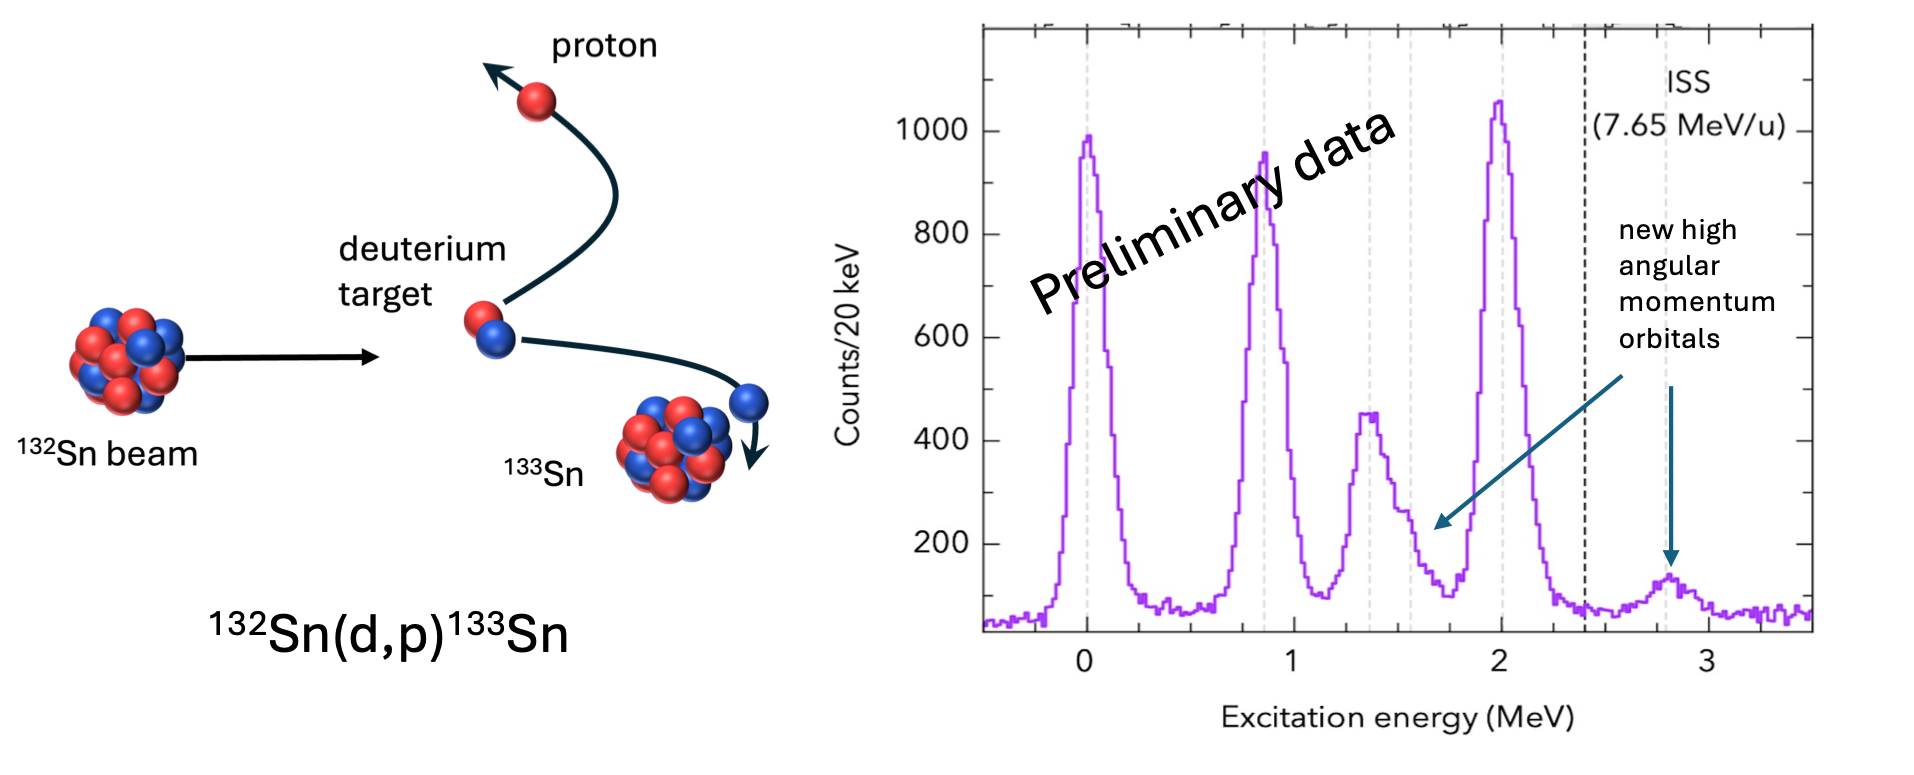
\includegraphics[width=0.9\linewidth]{graphics/ISOLDE_highlight_1.png}
    \caption{Left: A cartoon showing the mechanism for a direct \textit{(d,p)} reaction.
Right: A preliminary excitation spectrum for $^{133}$Sn showing peaks corresponding to the single-neutron states outside the N=132 core.
}
    \label{fig:ISOLDE_Highlight_1}
\end{figure}

Another project at GANIL/SPIRAL2 studied the \textbf{$^{12}$Be structure in the vicinity of different cluster thresholds}, such as $^4$He and $^8$He clusters using ACTAR-TPC detector (see Fig.~\ref{fig:2alpha_cluster}). 

\begin{figure}[!h]
    \centering
    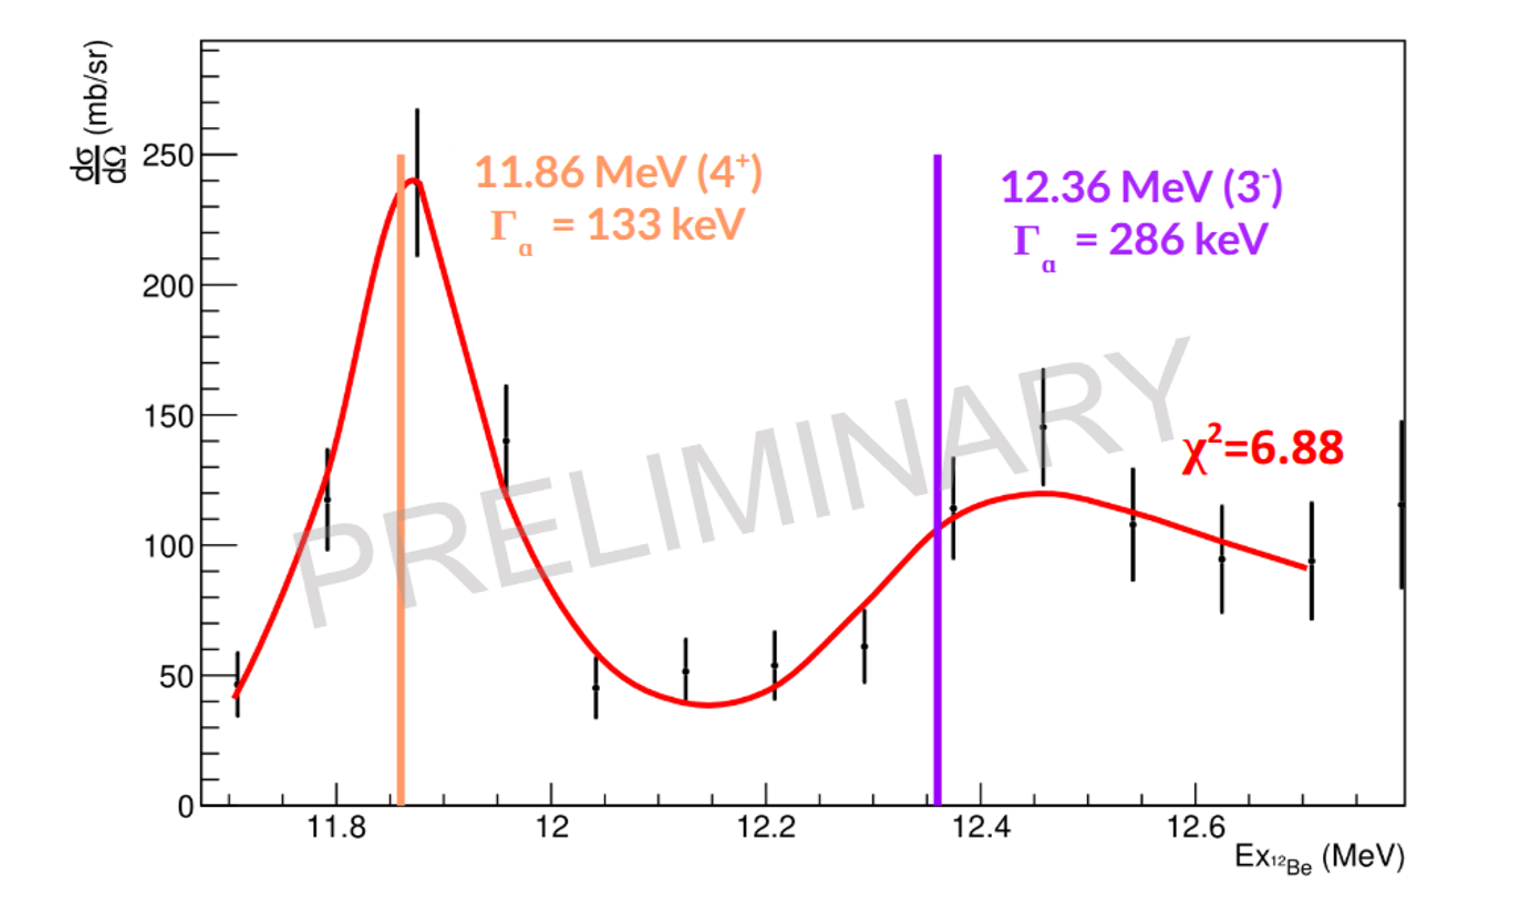
\includegraphics[width=0.6\linewidth]{graphics/2alpha_cluster.png}
    \caption{Two alpha cluster structure observed in $^{12}$Be by observing resonances in the resonance elastic scattering reaction $^4$He($^8$He,$\alpha$)$^8$He.The dark dots represents the experimental results, the red curve shows the quality of the theoretical decomposition of the results, while the violet and orange lines show the position of the cluster structure in $^{12}$Be.
}
    \label{fig:2alpha_cluster}
\end{figure}

In the project studied at JYFL joined a large collaboration from Spain (Valencia) and France (Subatech) at beta spectrometer after JYFLTRAP. This beta spectrometer has been used to directly measure the \textbf{shape of the beta spectrum of several fission fragments}. The motivation is connected to how well we understand the measured antineutrino spectrum from reactors.
%This was an excellent beam time, following on from an earlier run in 2022. Experimental improvements meant that the yields as well as the overall transmission (between 25-60\%) from the switchyard to the beta spectrometer were excellent. 
In total, around 14 cases of interest (including references) were measured, with 1 TB of data collected. These data will be sufficient to satisfy the needs of a large number of doctoral researchers in the near future.


\subparagraph{Task 2.3: Neutron Beams} \mbox{}

At the \textbf{n\_TOF} in CERN one project explored \textbf{new fission modes in lighter nuclear systems}, particularly cerium isotopes around atomic number 60 (Neodymium). Three other projects concentrated on neutron capture cross-section measurements for isotopes of Erbium and Neodymium (see Fig.~\ref{fig:n_TOF-146Nd})  improving accuracy in existing data. One of them specifically aimed to measure the $^{238}$U(n,$\gamma$) cross-section. Additionally, two projects investigated innovative techniques: measured neutron fluence using diamond detectors and testing the performances of a mixed array of HPGe and LaBr$_3$(Ce) detectors in beam.


\begin{figure}[!h]
    \centering
    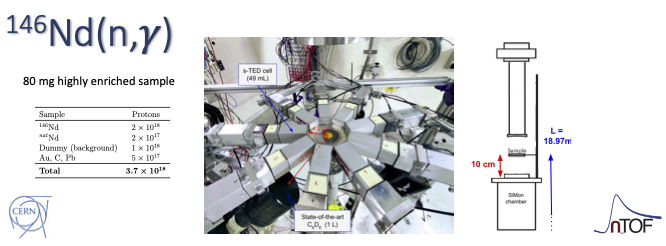
\includegraphics[width=1.0\linewidth]{graphics/n_TOF-146Nd.png}
    \caption{s-TED detector setup used at n\_TOF for the $^{146}$Nd(n,$\gamma$) reaction cross section measurement, one of the seven TA experiments executed with the EURO-LABS project support.}
    \label{fig:n_TOF-146Nd}
\end{figure}

In \textbf{CLEAR-CNA} a notable experiment was performed, measuring actinides in Baltic seaweed, characterizing novel targets for astrophysics, and assessing the impact of radioactivity from nuclear facilities. 

At the \textbf{ALTO} facility, one LICORNE project refined fast neutron tomography techniques and studied radiation damage in LaBr$_{3}$ crystals under high neutron fluence, crucial for the NUMEN project. 

At \textbf{GANIL}'s NFS facility, two key experiments investigated gas production in chromium and copper, respectively. Both projects utilized advanced experimental setups to measure double-differential cross sections for neutron-induced reactions, contributing valuable data for future fusion plant simulations and nuclear reaction models.

\subparagraph{Task 2.4: Theoretical Support} \mbox{}

The theoretical support offered at \textbf{ECT*} covered a broad range of subjects in various workshops, which were characterized by a high degree of interaction and collaboration among participants. At a fundamental level, progress has been achieved in the theoretical description of how quarks and gluons interact to give rise to the nuclear forces that shape the structure of nuclei. Strategies were mapped out to probe generalized parton distributions through novel exclusive processes and to use Lee-Yang singularities to determine the critical point of the QCD deconfinement transition. It was clarified that while global equilibrium in the QCD plasma probed in heavy-ion reactions is unique and independent of the pseudo-gauge choice, the definition of local equilibrium differs in quantum kinetic theory and quantum statistical field theory and is furthermore susceptible to a pseudo-gauge ambiguity. New directions have been charted for an {\it ab initio} development of optical potentials, including the Dispersive Optical Model and Green’s Function Theory, which are essential for the extraction of nuclear properties from lower-energy reactions. The takeaways for stellar dynamics, sensitivity studies, and astrophysical observations (including the determination of elemental abundances in stars) were extracted from key astrophysical reactions studied at facilities such as LUNA (Italy), JUNA and LEAF (China), CASPAR (USA), STELLA (France), Felsenkeller (Germany), and various large RIB installations. A Doctoral Training Program further enhanced the training of early career researchers in nuclear astrophysics, in particular the interplay between theory, experiment, and observations in the determination of the neutron-matter equation of state, as well as its impact on the neutron-star dynamics, neutrino emission, nucleosynthesis, and (gravitational and electromagnetic) signals from mergers. A separate workshop probed the extent to which these signals could provide a smoking gun for the presence of hyperons in neutron stars, which is strongly influenced by two- and three-body hyperon-nucleon forces inferred from information on hypernuclei. Nuclear theorists informed experimentalists of the specific data that is needed to benchmark and further develop models for neutrino-nucleus interactions, as needed for the analysis of next-generation oscillation experiments. Novel opportunities were identified for the determination of electric dipole moments, a sensitive probe of physics beyond the Standard Model of particle physics, such as a radioactive isotope/molecule program that could be envisioned at PSI (Switzerland). The nuclear physics opportunities of new high-power laser facilities, such as ELI-NP (Romania) have also been explored. Discussions on modern algorithms in machine learning and data analysis (from medical physics to research with accelerators and in underground laboratories) identified generative models at the LHC (Switzerland) as a promising strategy to reduce computing time, though challenges in deployment were acknowledged.

Overall, all of these initiatives of WP2 highlight significant advancements in nuclear physics research and the importance of collaborative efforts between theorists and experimentalists across various facilities.